\documentclass[a4paper,twoside]{article}

\usepackage{epsfig}
\usepackage{subcaption}
\usepackage{calc}
\usepackage{amssymb}
\usepackage{amstext}
\usepackage{amsmath}
\usepackage{amsthm}
\usepackage{multicol}
\usepackage{pslatex}
\usepackage{apalike}
\usepackage{algorithm2e}
\usepackage[bottom]{footmisc}
\usepackage[colorlinks=true,allcolors=blue]{hyperref}
\usepackage{todonotes}
\usepackage{SCITEPRESS}

\begin{document}
	
	\title{Next-generation design tools for intelligent transportation systems}
	
	\author{\authorname{Dominik Ascher\sup{1} and Georg Hackenberg\sup{2}}
		\affiliation{\sup{1}Faculty of Electrical Engineering and Computer Science, Technical University of Berlin, 10587 Berlin, Germany}
		\affiliation{\sup{2}School of Engineering, University of Applied Sciences Upper Austria, Stelzhamerstraße 23, 4600 Wels, Austria}
		\email{ascher@tu-berlin.de, georg.hackenberg@fh-wels.at}
	}
	
	\keywords{Model- and Simulation-based Systems Engineering}
	
	\abstract{Intelligent Transportation Systems (ITS) promote new transportation paradigms such as connected and autonomous vehicles (CAV), multi-modal and demand-responsive transport systems, and enable the transportation electrification by efficient operation of electric vehicles. Methods and tools are needed to explore the possible design space for emerging transportation paradigms, which support evaluation of system design alternatives and verification of system properties. In this work, we propose a modeling and simulation framework for capturing design decisions and evaluating emergent properties as well as control strategies for ITS design. In addition to capturing different design decisions, it assumes a user-centric perspective, where users can guide design decisions employing a novel user interface. We discuss and apply our modeling and simulation framework with respect to two specific applications.}
	
	\onecolumn \maketitle \normalsize \setcounter{footnote}{0} \vfill
	
	\section{Introduction}
	\label{sec:introduction}
	
	The transformative patterns of future mobility are enabled by interconnected and integrated systems and services.
	As such, Intelligent Transportation Systems (ITS) establish new transportation paradigms such as connected and autonomous vehicles (CAV), multi-modal and demand-responsive transport systems, as well as the transportation electrification by efficient operation of electric vehicles. In order to minimize environmental impacts \cite{kopelias2020connected}, complex scenarios between these systems and their requirements need to be holistically addressed, from which integrated system designs are derived, which enable transport infrastructures and their heterogenous actors to be efficient and sustainable.
	
	%Therefore, constituent systems need to be designed with respect to most efficient structures and control strategies within themselves, while accounting for and exploiting the emergent properties they achieve in conjunction and interdependence with other systems, as composed, integrated system-of-systems (SoS). 
	
	To systematically support the aforementioned systems engineering task, model- and simulation-based systems engineering~\cite{gianni2014modeling} can be employed for abstraction of design problems through the use of system models and their evaluation, i.e. their numerical approximation in terms of concrete behavior at run time. For this, well-defined system models are formulated at design time, for which then simulation aids projecting run-time information and performance metrics about the system under design and its environment. 

	However, as systems and their underlying requirements are typically imperfectly understood at the beginning of the design task, methods and tools are needed to explore the possible design space for emerging transportation paradigms, which support evaluation of system design alternatives and verification of system properties. 
	
	%As an effect of underspecified requirements, system models are often not completely understood, and modeling uncertainties need be adressed. 
	
	%Both structural as well as behavioral system design tasks can be supported using an overarching system design methodology at design time as well as at run time. 
	%In terms of benefits, on the one hand side, system models faciliate gaining improved system understanding through specification, while allowing rapid system modification through defined variation points for designing a system. On the other hand side, simulation aids approximating information about the system dynamics and performance of a system under design.
	For this, in previous work, we established an integrated systems modeling technique for integrated transportation and power systems, which allows one to model both transportation and power system scenarios, as well as mobility-on-demand scenarios to assess system design options systematically and improving system understanding holistically, based on a formal foundation~\cite{ascher_hackenberg_2014,ascher_hackenberg_2015,ascher_hackenberg_2016,ascher_hackenberg_2017}. The formal foundation was extended by a discrete event formalism \cite{ascher2023discrete} as well as integration with simulation tools and predictive models for control strategy optimization \cite{ascher_hackenberg_albayrak_2023}.
	
	\paragraph{Research objectives.}
	
	With our research, we want to help improve the efficiency and effectiveness of today's transportation systems.
	To achieve this goal, we work on methodologies for designing such systems and verifying their properties.
	Fundamentally, we promote a formal approach capturing the relevant design decisions and their relations.
	Furthermore, we integrate scenario-based simulation of system dynamics and evaluation of emergent properties.
	Finally, we exploit optimization algorithms for optimizing system dynamics as well as static design decisions.
	
	\paragraph{Research questions.}
	
	In this paper, we ask how the next generation of design tools for intelligent transportation systems should look like.
	Therefore, first we want to understand which system properties and design decisions should be represented in these tools.
	Then, we want to learn how the design decisions could be verified with respect to the desired system properties.
	Finally, we want to study how the relevant design information could be represented in a graphical user interface.
	
	\paragraph{Research methodology.}
	
	In the following, we first propose a modeling and simulation framework for capturing design decisions and evaluating emergent properties in Section~\ref{sec:approach}.
	%Then, we propose a graphical user interface for building system designs, starting simulation runs, and visualizing simulation outcomes in Section~\ref{sec:gui}.
	Thereafter, we propose two specific applications of our modeling and simulation framework as well as user interface technology in Section~\ref{sec:application}.
	Finally, we draw our conclusions and describe future direction of research and development on the design of ITS in Section~\ref{sec:conclusion}. 
	
	\section{Related work}

	This section provides an overview of related work, where we discuss infrastructure planning in Section 	\ref{sec:infrastructure-planning}, eco-routing and driving in Section \ref{sec:eco-routing}, cooperative driving in Section \ref{sec:cooperative-driving} as well as mobility-on-demand systems in Section \ref{sec:mobility-on-demand-systems}.

%	\subsection{Vehicle development}
%	
%	% Autonomous vehicles 
%
%	\textcolor{red}{Luftwiederstand Aussenhülle, Motorgeometrie (Computational Fluid Dynamics, Luftströmung, ...), Federungsverhalten (Multi-Body-Dynamics), Crashsimulation (Finite Element Analysis), Autonome Steuerung und Regelung (NVIDIA OMNIVERSE, Microsoft AIRSIM, CARLA Simulator)}
%	
%	For autonomous vehicle simulation, nvidia drive sim, CARLA \cite{dosovitskiy_carla_2017} and Airsim \cite{missing} are frequently used. .

	\subsection{Infrastructure planning}
\label{sec:infrastructure-planning}
	
	To investigate and simulate the travel behavior of transportation system users, traffic simulation may be used in order to support analysis and decision-making for transportation system engineering problems. In terms of the state-of-the-art, microscopic traffic simulation tools such as PTV Vissim \cite{fellendorf_vissim_1994}, MATSim \cite{w_axhausen_multi-agent_2016}, SUMO \cite{lopez_microscopic_2018} as well as AIMSUN \cite{barcelo2005dynamic} are well-established domain-wide. Typically, Origin-Destination matrics are used for modeling transportation demands.
	
	For instance, SUMO can be used to assess mesoscopic to microscopic traffic senarios. The infrastructure model of SUMO can separate between individual lanes for individual transport, defines intersections as well as traffic light controls. 
	
%	\textcolor{red}{Demand modeling and prediction (Origin-Destination-Matrix), Auswahl des Modalitätsmixes, Ladesäulen, Grob (Durchsatz) nach Fein (Spuren, Kreuzungen, Ampelschaltung)}

	\subsection{Eco-routing and -driving}
\label{sec:eco-routing}
	%\textcolor{red}{Fahrverhalten, Voraussschauendes Fahren, Aktueller Zustand des Verkehrsnetzes, Stauvorhersage, Strategien aus der perspektive eines einzelnen Fahrzeugen, nicht Kooperativ}

Eco-Routing describes a concept, which focuses on traffic participants, their routes and intermediate driving behavior in terms of targeting energy-efficient route selection and reduction of emissions, whereas the concept of Eco-Driving focuses on energy-efficient intermediate driving behavior \cite{ericsson2006optimizing,Boriboonsomsin2012}. For this, real-time and historical traffic information for routing and operation strategies to avoid congestions can be considered \cite{Boriboonsomsin2012}. However, if a single modality of transport is utilized excessively, compared to other modalities of transport, potential congestions may arise within transport networks of single modalities. Thus, energy-efficient utilization of all available transport modalities should be targeted within cross-system operation strategies and is enabled by the interconnection of everyday objects. 

	\subsection{Cooperative driving}
\label{sec:cooperative-driving}

	%\textcolor{red}{Platooning, Car2X (Vector CANoe Simulationsumgebung), fleet management}
	
	 The Internet of Things (IoT) refers to a term, which describes networked interconnection of everyday objects \cite{xia2012internet}, made possible by ubiquitous availability of sensor data from and actuation possibilities within physical objects being connected to the internet \cite{kopetz2011internet}. Here, Connected Mobility refers to an umbrella term for the potentially transformative patterns of future mobility made possible by interconnection of everyday objects. Examples include vehicular networking protocols such as Vehicle-to-Vehicle (V2V), Vehicle-to-Infrastructure (V2I) or Vehicle-to-Everything (V2X) communication protocols, but also concern specific use-cases such as vehicle platooning \cite{jia2015survey}, management of distributed electric vehicle fleets \cite{hu2016electric}, as well as using ICT for alignment of different transportation modalities \cite{harris2015ict}. Futhermore, use-cases integrating additional domains can be enabled such as using electric vehicle fleets to stabilize ancillary systems such as the power grid \cite{tomic2007using}.
	
	 In terms of co-simulation approaches, Eclipse MOSAIC \cite{noauthor_eclipse_nodate} is an open architecture for multiscale simulations for smart and connected mobility. Originally intended to simulate V2X interactions \cite{schunemann_v2x_2011}, integrations with SUMO, as well as autonomous vehicle simulation tools such as CARLA \cite{dosovitskiy_carla_2017} have been proposed. Here, based on MOSAIC, Cui et al. \cite{cui_extensible_2023} propose an extension to the simulation tool CARLA for investigation of cooperative driving scenarios. 
	
	\subsection{Mobility-on-demand}
\label{sec:mobility-on-demand-systems}
	%\textcolor{red}{rebalancing, ride sharing, ride hailing, multi-modality}
	Mobility-on-demand systems refer to systems, where the transportation demand gets covered by a set of different transportation modalities, which make up the transportation supply.
	Canzler et al. \cite{canzler2016mobility} argue the close link of modernity and private car use is beginning to dissolve. Particularly, inter-modality and variable modes of transport are becoming more important for urban development \cite{rode2015towards}. New transportation models such as ridesharing favor shared mobility over personal mobility, and bring together passengers with a shared route in shared vehicles \cite{cohen2014ride}. For instance, prospective control strategies for ridesharing systems have been established in \cite{furuhata2013ridesharing,agatz2012optimization}.
	 In this context, autonomous vehicles enable the idea of \textit{autonomous mobility-on-demand} systems, where fully-autonomous transportation modalities, i.e. autonomous vehicles, effectively cover transportation supply, whose control strategies have shown to provide interrelated benefits for the transportation system in terms of increased efficiency \cite{fagnant2014travel}. However, autonomous mobility-on-demand systems introduce the challenge of distributing a supply of autonomous vehicles in a given area to cover passenger transportation demands evenly. Thus, developed control strategies have to balance transportation supply with transportation demands, while not becoming skewed towards the most popular origins and destinations of demands \cite{pavone2012robotic,zhang2016control}. In addition, besides passenger transport, freight transport has to be considered within mobility-on-demand systems, as for instance, in urban environments, freight movements are main drivers of pollution  \cite{amaral2015city}. %In turn, according systems can be used to optimize supply-chains, thereby providing added value in terms of decreased transport costs. 
	
	\section{General approach}
	\label{sec:approach}
	
	In this section, we propose a modeling and simulation framework for the design of intelligent transportation systems.
	We first introduce the scope and intended usage of the framework in Section ~\ref{sec:scope}.
	Secondly, we present the methodology for describing design decisions in Section~\ref{sec:methodology}.
	Thirdly, we describe the domain-specific concepts our modeling and simulation framework employs for designs in Section~\ref{sec:domain-specific-modeling}.
	%Then, we propose an interface for implementing and integrating custom control strategies in Section~\ref{sec:controller-interface}.
	%Finally, we define an interface for collecting statistics during simulation of system dynamics in Section~\ref{sec:statistics-interface}.
	
	\subsection{Intended usage}
	\label{sec:scope}
%	\begin{figure}[!ht]
%		\missingfigure{Designer input + output}
%		\caption{TODO}
%	\end{figure}
	
	Our approach is based on integrated transportation system modeling techniques, which allow assessment of integrated, electrified ITS systems for the purpose of designing emergent integrated system properties.
	
	In terms of scope, our modeling technique supports both static property, i.e. structural and infrastructure design, and dynamic property design, i.e. behavior and control strategy design. For this, we subsequently consider a set of different roles including transportation system engineers, charge point operators as well as mobility fleet operators. For each of the roles, we briefly describe exemplary use-cases for our system modeling technique in terms of static as well as dynamic property design.

\subsubsection{Transportation System Engineer}
Transportation system engineers are responsible for maintaining and designing the transportation infrastructure.

%Wo setzte ich Kreuzungen? Wo sollen Straßen verlaufen? Wie breit sollen die Straßen sein?urban traffic control

\begin{itemize}
	\item \textbf{Static Properties:} In terms of devising static properties, transportation system engineers are supported in the investigation of transportation infrastructure properties such as determing optimal transportation links between different locations such as placement of intersections and roads. In addition, transportation capacities of transportation links such as number of lanes may be considered as well.
	\item \textbf{Dynamic Properties:} For determining dynamic properties instead, transportation system engineers may be supported in determining control strategies for urban traffic control such as cycle times for traffic lights based on expected transport demands. 
\end{itemize}
	
\subsubsection{Charge Point Operators}
Charge point operators are responsible for maintaining and operating a set of charging station in a defined area, i.e. the charging station infrastructure. 

\begin{itemize}
	\item \textbf{Static Properties:} In terms of determining static properties, charge point operators may be supported in devising charging infrastructure such as placement of charging stations along most popular routes and points of interest. 
	\item \textbf{Dynamic Properties:} In terms of determining dynamic properties, control strategies may be devised for future transportation electrification scenarios. This includes distributed charging coordination between multiple charging stations during times of increased charging demands as well as coordinated utilization of renewable energy sources and self-sufficiency.
\end{itemize}
%Wo sollen Ladestationen sein?

\subsubsection{Mobility Fleet Operators}
Mobility fleet operators are responsible for coordinating and managing a fleet of vehicles under their supervision, which is able to serve transportation demands. 

\begin{itemize}
	\item \textbf{Static Properties:} To devise static properties, moblity fleet operators are supported in determination of fleet capacity as well as determination of used vehicle types.
	\item \textbf{Dynamic Properties:} For devising dynamic properties instead, mobility fleet operators are supported by investigated demand-responsive transport scenarios. This includes determing routing and driving behaviors for the mobility fleet with respect to underlying goals such as energy-efficiency or shortest traveling times. Furthermore, optimal assignment of transportation demands to available transportation capacities in the context of on-demand transportation problems is supported as well.
\end{itemize}
	
	%Wieviele Fahrzeuge soll meine Flotte umfassen? Welche Fahrzeugklassen? Welche Fahr und Routing Strategien?
	
		
	\subsection{Design methodology}
	\label{sec:methodology}

	%\textcolor{red}{Formal, Probabilistic}
	
	% Simulation-based Approach
	Our approach employs model- and simulation-based systems engineering~\cite{gianni2014modeling} for decision-making with respect to system designs for the ITS domain.
	Models are described based on the problem domain, where simulation aids obtaining information about designs of the solution domain. 
	% Scenario-based
	For the latter, we employ a scenario-based approach, where a set of requirements is typically mapped from and to scenarios \cite{sutcliffe_supporting_1998}. Figure \ref{fig:concept} shows an overview of the system design methodology.
	
	% TODO Figure
	\begin{figure}[!ht]
		\centering
		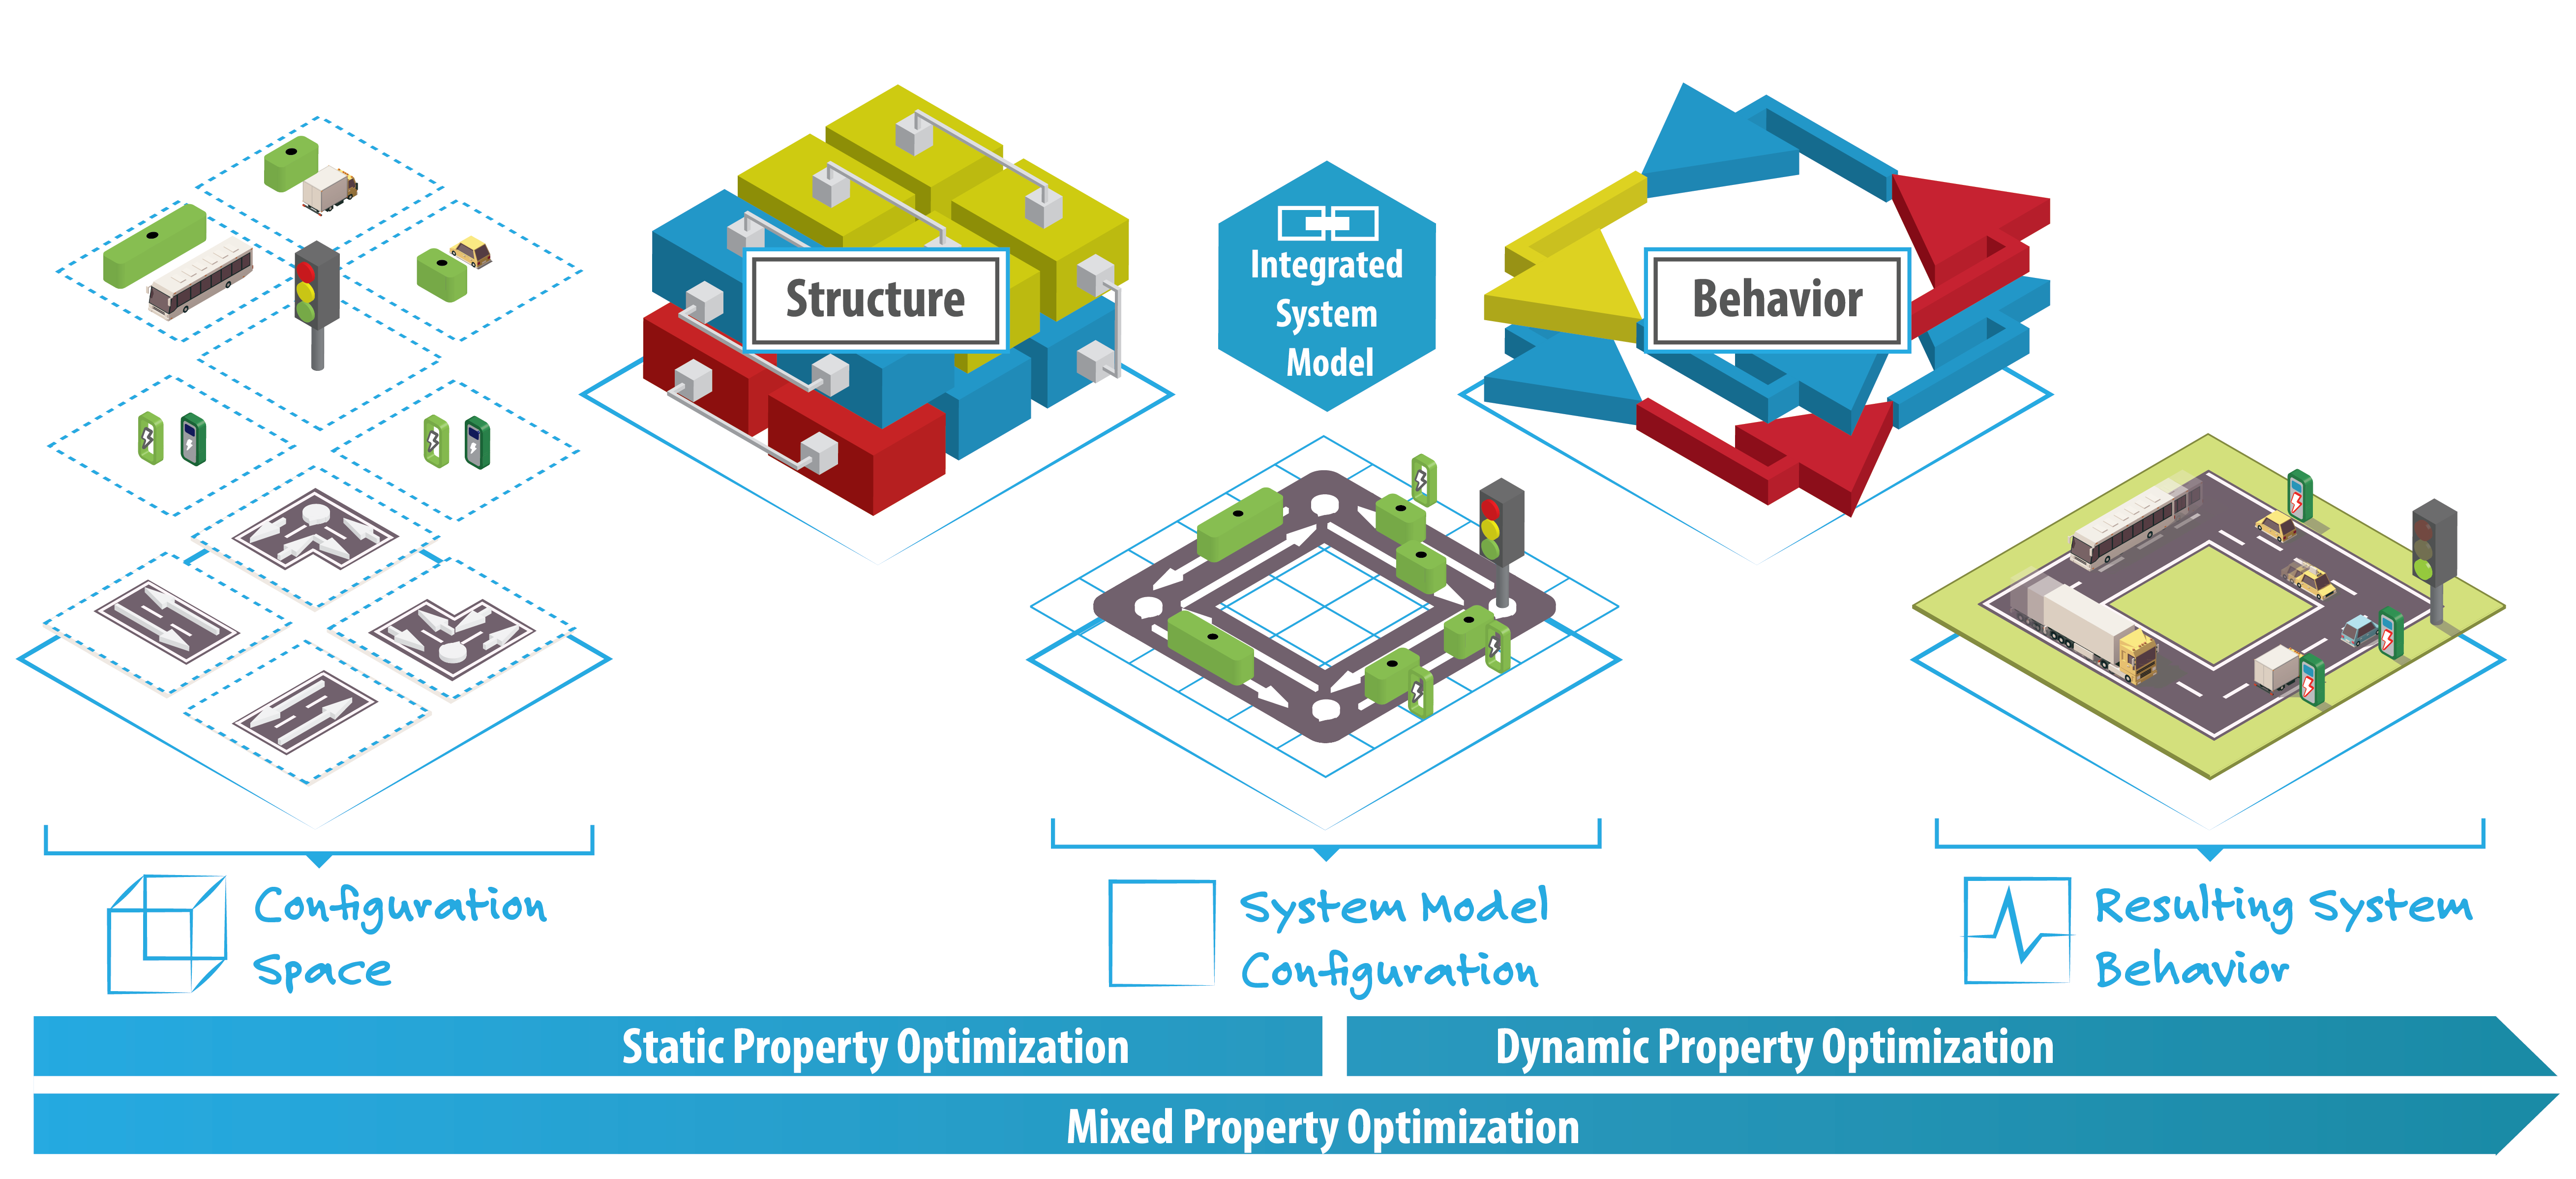
\includegraphics[width=1.0\columnwidth]{property_optimization.png}
		\caption{System design methodology}
		\label{fig:concept}
	\end{figure}
	
	% Formal foundation
	\subsubsection{Problem Formulation}
	For system models, each concept is described in terms of their static (i.e.\ time-independent) properties and calculations as well as their dynamic (i.e.\ time-dependent) properties concerning state evolution during simulation including states and actions. In addition, we describe requirements of a system design in terms of contribution functions as well as constraint functions, which are mapped to static or dynamic properties.
	
	In terms of static properties, we define a one-tuple $(COM)$ consisting of the components, as well as their parameters and configurations, which we describe subsequently:
	\begin{itemize}
		\item Component. The core element of the underlying systems modeling technique is the \textit{component}, where components are denoted by $com \in COM$. 
		\item Parameters. Parameters describe static information about components which does not change based on dynamic behavior, i.e. time steps.
		\item Configurations. Components are configured with respect to specific sets of parameters by using within \textit{configurations} $\mathcal{COM}_{conf}: COM$. Here, a configuration refers to a specific set of \textit{parameters}. For example, a configuration for a component $com_{id}$ containing a single parameter $com_{param} \in \mathbb{D}$, with arbitrary domain $\mathbb{D}$, could be defined as a mapping $\mathcal{COM}_{conf}: COM \rightarrow \mathbb{D}$.
		
		
	\end{itemize}
	
	
	For dynamic properties, we define the four-tuple $(S, A, T, E)$, consisting of the sets of states $S$, actions $A$, transition functions $T$ and events $E$, which we describe subsequently:	
	\begin{itemize}
		\item State variables $S_t$ constitute the states at time $t$ within a state space of all possible states $S$ such that $S_t \subset S$. Here, the state variables describe a vector of system or observable environment variables at a given time instant. 
		\item Action variables $a_t$ describe the actions available to choose from at time $t$ within a discrete action space $A$ such that $a_t \subset A$. Actions $a_t$ depend on the state variables $S_t$ as indexed by time $t$.
		\item Transition functions $T$ describe how one state $S_t$ at time $t$ evolves to another state $S_{t+1}$ at time $t+1$, given an action $a_t$. Transition functions describe a mapping such that $T : S \times A \to S$. 
		\item Events $E$ are defined as functions over a system's trajectory of states, which indicate when actions need to be taken in the system simulation. They describe a mapping $E : S \to A$. 
	\end{itemize}
	
	% Objectives, Constraints, Actions, 
	The parameters and actions \textit{which} need to be taken are determined based on a set of requirements, where we define objectives as contribution functions, as well as constraint functions. Thus, we define the tuple $(C, CSF)$, which is subsequently described:
	
	\begin{itemize}
		\item Contribution functions $C$ describe a numerical value for being in a state $S_{t}$ while taking action $a_{t}$ in a particular time instant $t$. Here, a contribution function is a mapping $C : S \times A \to \mathbb{R}_0$.
		%Note that, in this context, $costs$ can be formulated as negative contributions instead.
		\item Constraint functions $CSF$ describe mappings such that $CSF : S \times A \to \mathbb{B}$ with Boolean set $\mathbb{B} = \{\mathit{true},\mathit{false}\}$, and therefore restrict admissable, i.e. valid, states and actions. 
	\end{itemize}
	
	\subsubsection{Problem Solution}
	The design problem then consists in determining the set of states and actions which conform to the imposed objectives and constraints. 
	
	%Monte-Carlo-Simulation
	For solving according design problems, Dynamic Programming \cite{bellman_dynamic_1957} methods might be used for small-scale problems, which iteratively explore the state space to find an optimal solution, where such a problem is solved over a defined time horizon $[t_0,T]$, i.e. from initial time increment $t_0$ to the final time increment $T$. For this, the \textit{value function} $V_t(S_t)$ has to be calculated for each value of $S_t$, and consists of all aggregated contributions over time, where a discount factor $\gamma$ for scaling the value of future contributions is usually employed. Then, the optimal value function $V_t$ refers to the longterm value of being in state $S_t$ in time $t$ and is a mapping $V : S \times A \times S \to \mathbb{R}$, such that
	\begin{equation}
		V_t(S_t) = \max_{a_t}\ C_t(S_t,a_t) + \gamma \sum_{S_t \in S}^{}V_{t+1}(T(S_t,a_t)) \mathrm{.}
	\end{equation}
	
	Then, a \textit{policy function} can refer to any method for determining an action, given a state. For instance, a deterministic policy function $\pi$ can be defined as a mapping such that $\pi : S \to A$, where each state is mapped to an action. Note that probabalistic formulations for policy functions are possible as well.
	To solve the problem using classic dynamic programming, an optimal \textit{policy function} $\pi^* : S \to A$ has to be introduced, which chooses an action $a_t \in \mathit{A_t}$ resulting in the highest contribution at every time step, thereby maximizing the value function over time, i.e. $\textit{for each} \enskip S_t \in S:$
	\begin{equation}
		\pi^*(S_t) = \arg \max_{a_t}\ C_t(S_t,a_t) + \gamma \sum_{S_t \in S}^{}V_{t+1}(T(S_t,a_t)) \mathrm{.}
	\end{equation}
	
	However, Dynamic Programming methods are subject to increasing problem complexity with increasing dimensionality of parameter, state and action spaces, i.e. the curse of dimensionality \cite{bellman_dynamic_1957}, and are therefore not scalable for complex problems.
	
	Due to this, the whole state, action and parameter space cannot be iterated for complex problems due to expontially increasing problem complexity and limited computional resources. 
	To reduce simulation complexity we apply the following methods:

\begin{itemize}
	\item Discrete-Event Simulation. As simulation complexity increases with the number and dimensionality of considered parameters, states, and actions of modeled systems, our approach employs Discrete-Event Simulation (DES)~\cite{fishman2001discrete}, where events are defined as functions over a system's trajectory of states, which indicate \textit{when} actions need to be taken in the system simulation.	Thus, simulation complexity is reduced by limiting action space dimensionality and by abstracting from discrete-time resolutions~\cite{ascher2023discrete}.
	\item Monte-Carlo Simulation. In addition, Monte-Carlo methods are used, which partially and/or randomly \textit{sample} the state space until an sufficient number of samples is reached for exploration to limit problem complexity. 
\end{itemize}

As noted, a policy function $\pi$ may be a simple function or may involve extensive computation as a search process \cite{mania2018simple}. To reduce policy function computation complexity we apply the following methods:
\begin{itemize}
	%Heuristic Search
	\item Heuristic Search. Here, the policy function is defined as a heuristic search procedure, which is iteratively designed by a domain expert, which uses simulation results to adapt heuristic control logic as needed. 
	% Approximate Dynamic Programming
	\item Approximate Dynamic Programming. Alternatively, approximations of the policy as well as value functions may be automatically derived. Here, Approximate Dynamic Programming (ADP) methods \cite{powell_approximate_2007} are used, which aim to approximate policy and/or value functions to reduce problem complexity. 
\end{itemize}

	\subsubsection{Application to Design Problems}
	Based on the described concepts, our approach supports different design tasks, where evaluation of designs is performed using approximate and heuristic optimization techniques. We utilize optimization to evaluate solutions for the following design problems:

	\begin{enumerate}
		% Configuration Space (Parameters)
		\item \textbf{Static property optimization} concerns static design decisions such as optimization of transportation infrastructure properties. For this, the methodology assumes a \textit{configuration space}, which describes components, their parameters, as well as connection possibilities between components. From the configuration space, components are instantiated using concrete parameters, which are determined based on requirements, i.e. objectives and constraints, thereby creating a structure. The outcome of static property  optimization describes a system model configuration.
		% State space
		\item \textbf{Dynamic property optimization} concerns dynamic design decisions, i.e. optimization of control strategies such as determining efficient transportation entity behavior. This task involves exploring the state space of a system model configuration based on a set of requirements, where the outcome is a control strategy. Here, control strategy engineering involves determining trajectories of states and actions which conform to imposed requirements, i.e. goals and constraints. 
		\item \textbf{Mixed property optimization} concerns the integrated design task for optimization of both static and dynamic design decisions. Thus it describes the integrated task which involves both static and dynamic property optimization.
	\end{enumerate}
	
	%In addition, relationships between components can be incorporated by specifying well-defined component interfaces and their connection.
	
	%\subsubsection{System Theory}
	%\label{sec:system-theory}
	
	\subsection{System theory}
	\label{sec:domain-specific-modeling}
	
	%Figure~\ref{fig:modeling-technique} provides an overview of main domain concepts, where the formalism is intended to capture a concise and an essential set of static properties, static calculations, and dynamic states as well as events for establishing sound models and control strategies for on-demand transportation systems. For details on the underlying modeling concepts, we refer to \cite{ascher2023discrete}. Subsequently, we describe a brief overview of these concepts.
	
	On a domain-specific modeling level, the approach allows modeling integrated transportation system problems on mesoscopic to microscopic levels, \cite{ascher_hackenberg_2014,ascher_hackenberg_2015}, supported by a formal systems modeling foundation \cite{ascher_hackenberg_2016,ascher_hackenberg_2017} (See Section  \ref{sec:scope}). 
	Figure \ref{fig:domain-specific-modeling} shows an overview of the domain-specific modeling concepts. In the following, we provide a brief overview of domain concepts, states, as well as events, where we refer to \cite{ascher2023discrete} for a detailed overview. 
	% TODO Figure
	\begin{figure}[!ht]
		\centering
		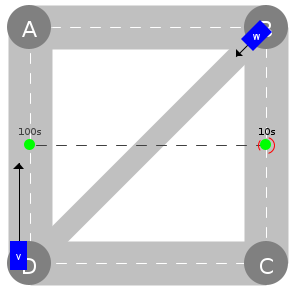
\includegraphics[width=0.6\columnwidth]{../../events/demand.png}
		\caption{Domain-specific modeling concepts.}
		\label{fig:domain-specific-modeling}
	\end{figure}
	
	\paragraph{Concepts}
	
	Considered domain concepts for the formalism include intersections $i \in I$, segments $s \in S$ as well as locations $l \in L$ for describing properties about the transportation infrastructure.
	Based on the transportation infrastructure, we use charging stations $cs \in CS$ for describing the charging infrastructure. Furthermore, we use vehicles $v \in V$ to describe the transportation supply and capacities. Transportation demands $d \in D$ are based on the transportation infrastructure, and temporarily consume available transportation capacities such as vehicles.
	
	\paragraph{States}
	Based on the described domain concepts, we describe dynamic (i.e. time-dependent) state functions for charging stations $S_{CS}$, demands $S_{D}$, as well as vehicles $S_V$:
	
	\begin{itemize}
		\item In terms of charging station states $S_{CS}$, we describe the current vehicle which is connected to the charging station $S_{CS.CV}$, as well as the current charge speed $S_{CS.CCS}$.
		\item In terms of demand states $S_{D}$, we describe the current vehicle carrying the demand $S_{D.CV}$, as well as the current location of the demand $S_{D.CL}$.
		\item For vehicle states $S_{DV}$, we describe the current battery level of the vehicle $S_{V.CBL}$, the current location of the vehicle $S_{V.CL}$, as well as the current drive speed of the vehicle $S_{V.CDS}$.
	\end{itemize}
	
	\paragraph{Events}
	We define the following domain-specific events $E$:
	%	Events $E$ are defined as functions over a system's trajectory of states, which indicate when actions need to be taken in the system simulation. For this, we define the following events:
	\begin{itemize}
		\item Events indicating when vehicles arrive at an intersection $E_{V.AI}$ or when vehicles depart at an intersection $E_{V.DI}$ to derive routing decisions. 
		\item Events indicating when vehicles arrive at a charging station $E_{V.ACS}$ to derive charging decisions. 
		\item Events indicating when vehicles arrive at a demand pick-up location $E_{V.ADP}$ and when vehicles arrive at a demand drop-off location $E_{V.ADD}$ to derive demand pick-up and drop-off decisions. 
		\item Events indicating when vehicles arrive at another vehicle on the same segment, including a faster vehicle arriving at a  slower vehicle $E_{V.AVS}$, as well as a faster vehicle departing at a slower vehicle $E_{V.DVS}$ to derive overtaking decisions.
		\item Events indicating when a demand appears $E_{D.AD}$ to derive decisions for vehicles to serve demands.
		\item Events indicating when vehicles change their drive speed $E_{V.CDS}$ and when vehicles change their charge speed $E_{V.CCS}$ to derive decisions for overtaking and charging behaviors. 
		\item Events indicating when vehicles batteries are either empty $E_{V.CBE}$ or vehicles batteries are full $E_{V.CBF}$ to derive decisions for stopping driving and charging behaviors.
	\end{itemize}

	%\paragraph{Constraints}
	
	\section{Tool prototype}
	\label{sec:tool-prototype}
	
	Based on the general approach explained in Section~\ref{sec:approach} we started developing an open source tool prototype hosted on GitHub\footnote{\url{https://github.com/ghackenberg/transport-ide}}.
	The tool prototype is written in Java\footnote{\url{https://docs.oracle.com/javase/tutorial/java/}} and uses the Swing library\footnote{\url{https://docs.oracle.com/javase/tutorial/uiswing/}} as well as the JFreeChart library\footnote{\url{https://www.jfree.org/jfreechart/}} for visualization.
	Furthermore, the prototype uses the JGraphT\footnote{\url{https://jgrapht.org/}} library for computing shortest paths in the road network.
	
	In the following, we explain several interesting aspects of the tool prototype:
	In Section~\ref{sec:data-model} we dive into the core data structures for representing both static system configurations as well as dynamic system states.
	Then, in Section~\ref{sec:controller-interface} we explain how the users can implement and integrate different control strategies into the tool prototype.
	Next, in Section~\ref{sec:statistics-interface} we describe the data, which is collected during simulation runs and which can be used for visualizations and possibly training.
	Thereafter, in Section~\ref{sec:simulation-engine} we provide an overview of the engine, which computes the discrete events and updates the system states accordingly.
	Finally, in Section~\ref{sec:application} we highlight two different applications, which we have implemented already based on the previous framework elements.
	
	%Figure~\ref{fig:software-architecture} illustrates the module architecture of the tool prototype.
	%The architecture consists of the eight modules \texttt{model}, \texttt{controller}, \texttt{statistics}, and \texttt{simulator} as well as \texttt{parser}, \texttt{exporter}, \texttt{viewer}, and \texttt{program}.
	
	%\begin{figure}[!ht]
	%    \centering
	%    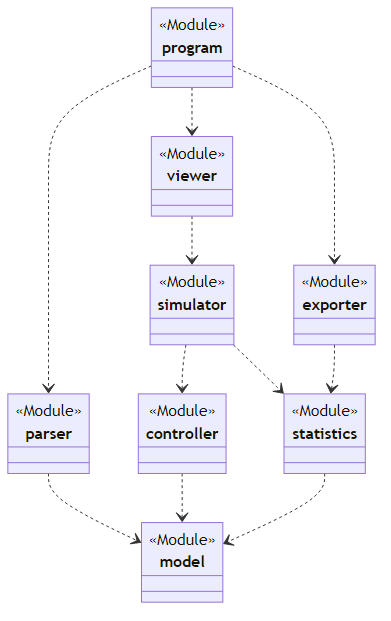
\includegraphics[scale=0.4]{../../diagrams/architecture-v2.png}
	%    \caption{Modular software architecture.}
	%    \label{fig:software-architecture}
	%\end{figure}
	
	%In the following, we discuss each module in more detail including their resposibilities and dependencies on the other modules.
	
	\subsection{Data structures}
	\label{sec:data-model}
	
	The \texttt{model} module provides the core data structures for modeling static system configurations and representing dynamic system states.
	Figure~\ref{fig:data-model} shows the classes, their attributes, and their relationships.
	
	\begin{figure}[!ht]
		\centering
		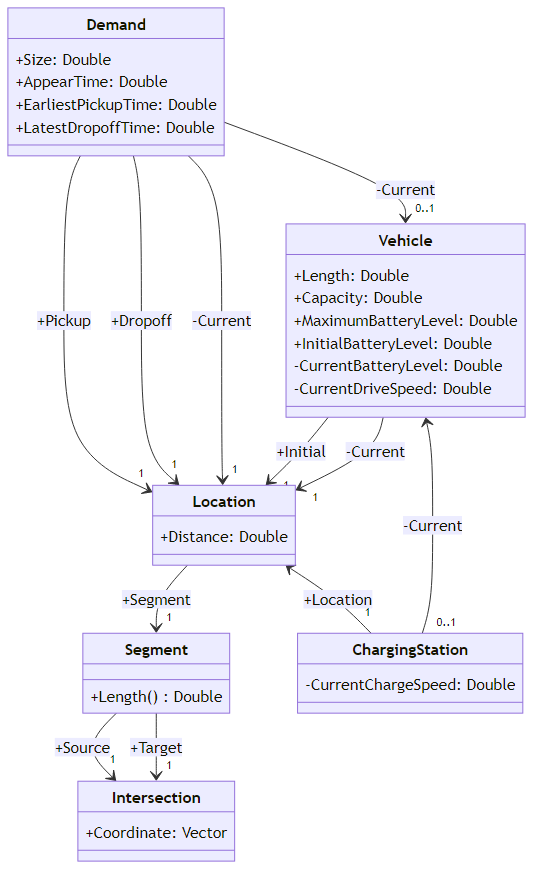
\includegraphics[scale=0.4]{../../diagrams/model/classes-v0.2.png}
		\caption{Configuration and simulation data model.}
		\label{fig:data-model}
	\end{figure}
	
	The \texttt{Intersection} class represents intersections of the driving infrastructure.
	Each intersection stores its coordinate in three-dimensional space.
	Note that we use Cartesian coordinates for simplicity.
	
	The \texttt{Segment} class represents road segments of the driving infrastructure.
	Each segment points to its source and its target intersection.
	Furthermore, each segment provides a method for computing its length.
	Note that we use the Euclidean distance between source and target intersection here.
	
	The \texttt{Location} class represents specific points on the segments of the driving infrastructure.
	Each location points to the corresponding segment of the driving infrastructure.
	Furthermore, each location stores a distance on this segment.
	The distance is measured in Eclidean units of the Cartesian space.
	
	The \texttt{ChargingStation} class represents the charging infrastructure.
	Each charging station stores its location on the driving infrastructure.
	Furthermore, each charging station optionally points to a current vehicle.
	Then, each charging station provides the current charging speed.
	Note that the simulator computes the current charging speed dynamically.
	
	The \texttt{Vehicle} class represents the driving resources.
	Each vehicle provides an initial and a current location on the driving infrastructure.
	The initial location defines the position of the vehicle in the initial state of the simulation.
	Then, the simulator continuously updates the current location of the vehicle.
	Furthermore, each vehicle stores a length and a capacity, a maximum, an initial, and a current battery level, and a current drive speed.
	The length determines how much space the vehicle occupies on the driving infrastructure.
	The capacity defines how much demand the vehicle can carry.
	The maximum battery level specifies the size of the energy storage.
	And the initial battery level stores the load state of the enery storage at simulation start.
	Finally, the simulator continuously updates the current battery level as well as the current drive speed.
	
	The \texttt{Demand} class represents the transportation loads to be served.
	Each demand points to a pickup and a dropoff location as well as a current location and vehicle.
	Furthermore, each demand stores a size as well as an appear, and earliest pickup, and a latest dropoff time.
	The simulator continously updates the current location and vehicle.
	
	\subsection{Control strategies}
	\label{sec:controller-interface}
	
	%For evaluation of defined system designs, the approach offers an controller interface for defining control strategies. 
	
	During a simulation run, a number of control decisions have to be taken.
	For example, when arriving at an intersection each vehicle has to select the next outgoing road segment.
	Similarly, when arriving at a demand pickup location each vehicle as to decide whether to serve the demand or not.
	The overall system performance heavily depends on the optimality of the individual choices made during a simulation run.
	Therefore, one key engineering task for this class of systems is to develop an appropriate control strategy.
	Since the desired control strategy cannot be hardcoded upfront, the simulator supports plugging in and testing different strategies.
	Each control strategy must implement the controller interface methods depicted in Figure~\ref{fig:controller-interface}.
	
	\begin{figure}[!ht]
		\centering
		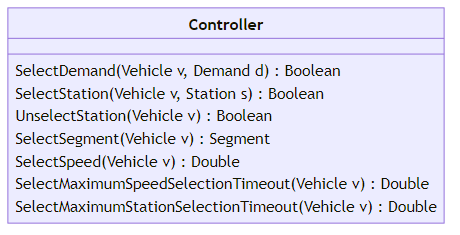
\includegraphics[scale=0.4]{../../diagrams/controller/classes-minimal.png}
		\caption{Methods of the controller interface.}
		\label{fig:controller-interface}
	\end{figure}
	
	For tool demonstration and evaluation purposes, we currently provide four different implementations of the controller interface: A \textbf{manual}, a \textbf{random}, a \textbf{greedy}, and a \textbf{smart} control strategy.
	Figure~\ref{fig:control-strategies} provides an overview of the four control strategies and their decision logic.
	The columns of the matrix represent the individual control strategies, the rows represent the decisions to be taken, and the cells represent the corresponding logic.
	
	\begin{figure}[!ht]
		\centering
		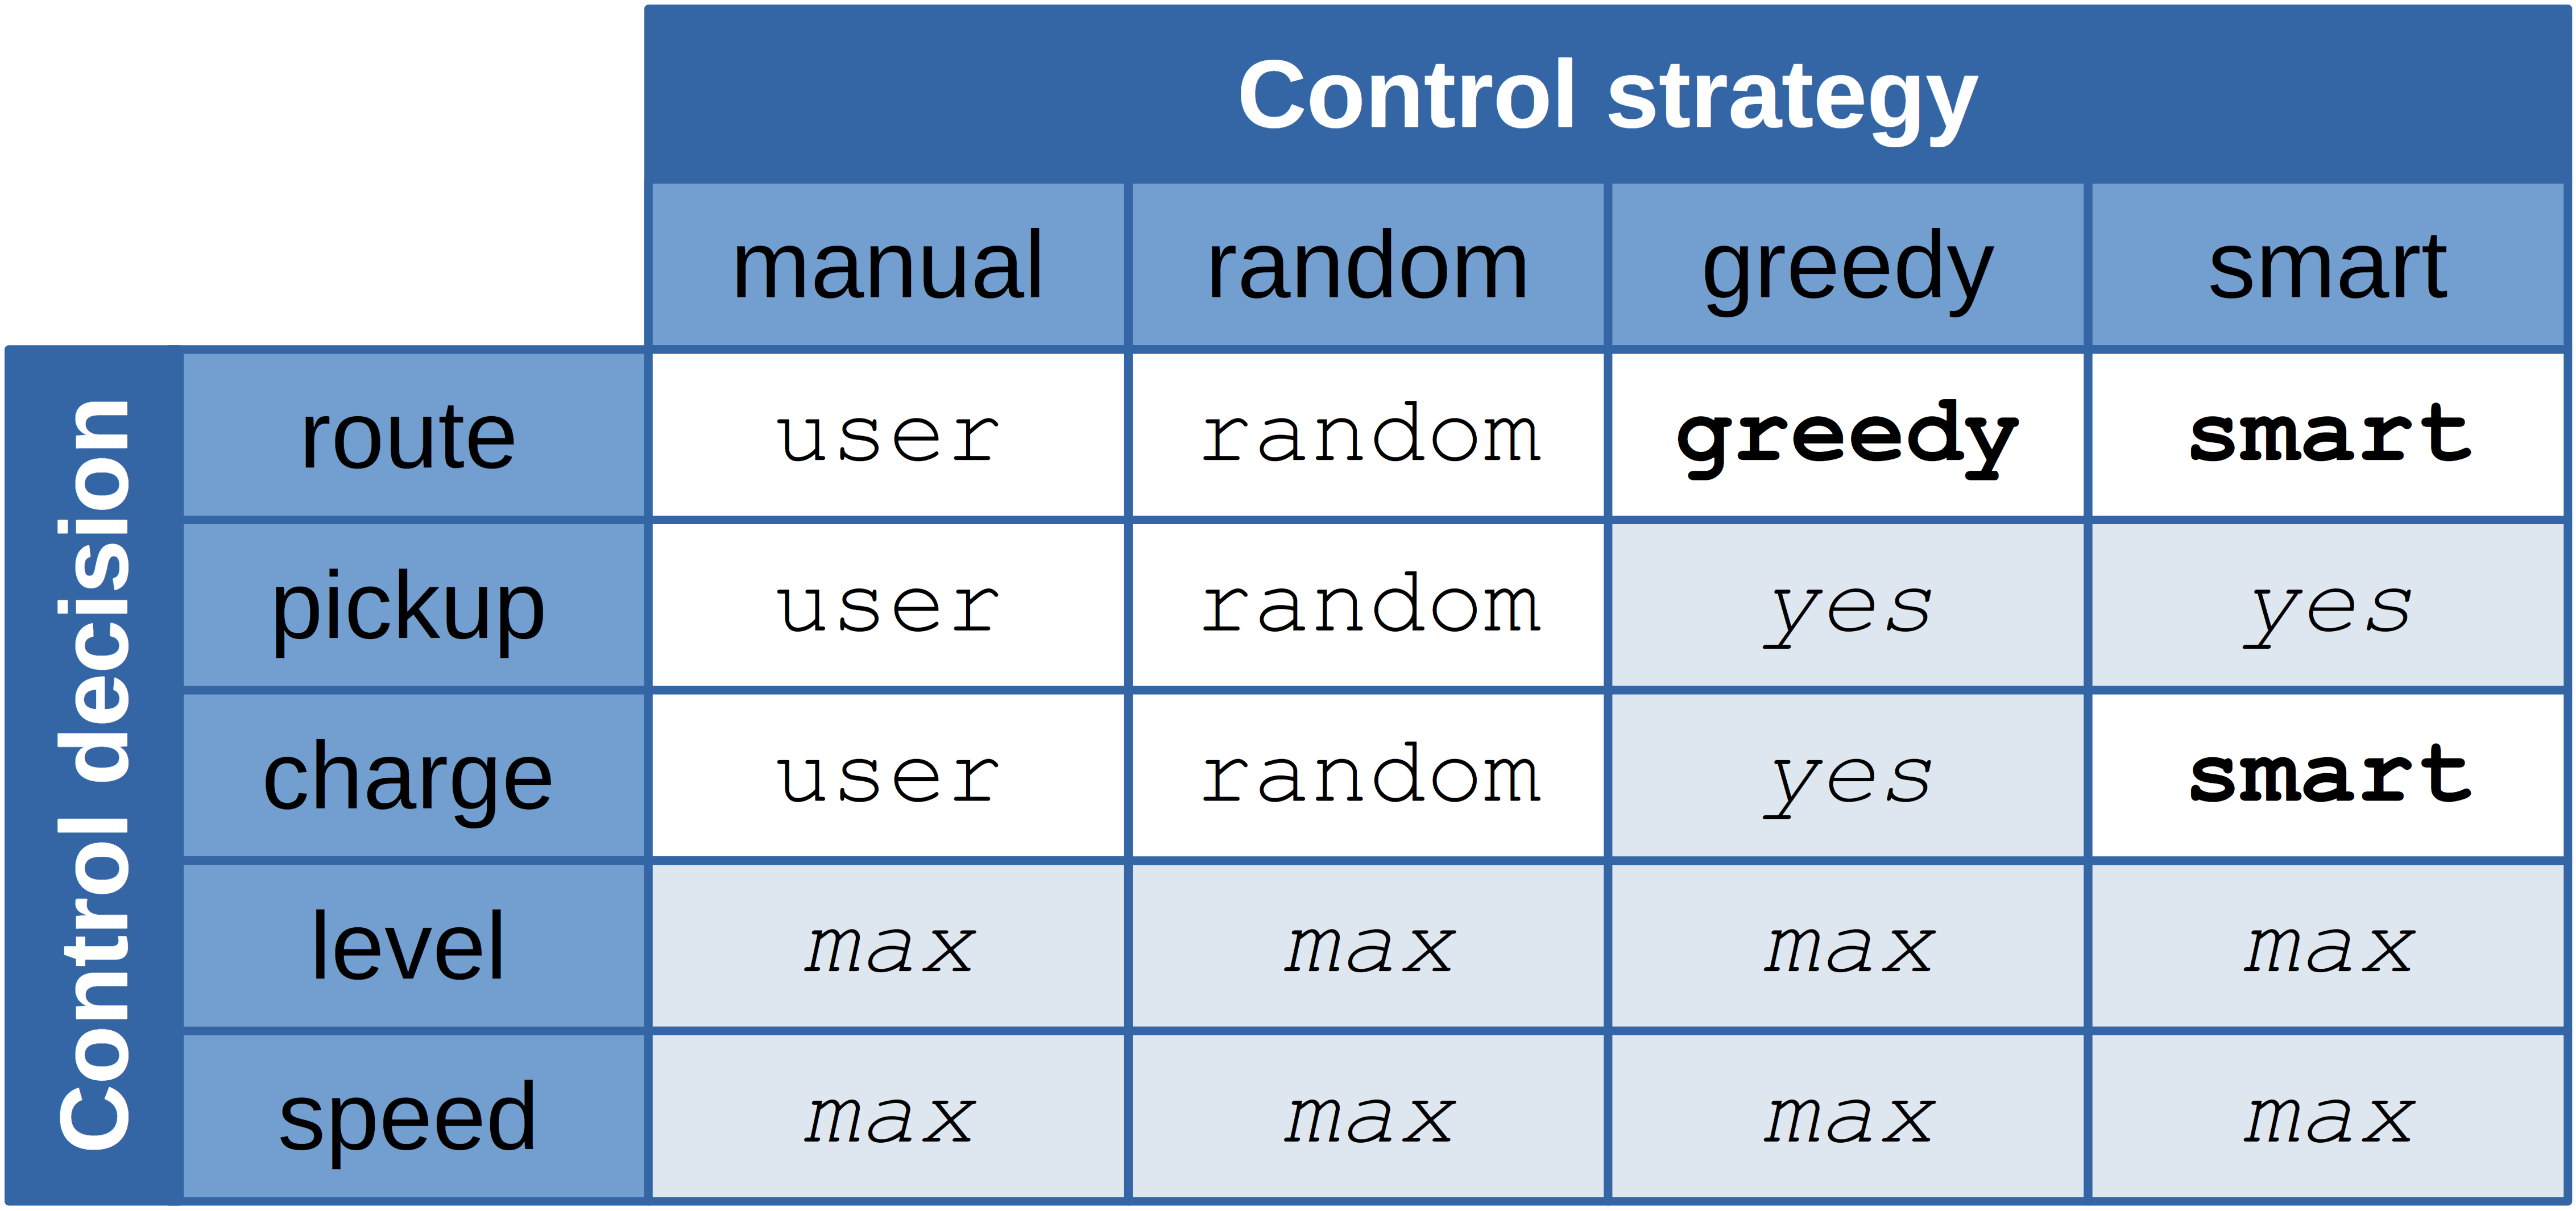
\includegraphics[width=0.8\columnwidth]{control_strategy_overview.png}
		\caption{Overview of the control strategies.}
		\label{fig:control-strategies}
	\end{figure}
	
	In the following, we describe the logics behind each of the control strategies in more detail.
	
	\subsubsection*{Manual control strategy}
	\label{sec:controller-manual}
	
	The manual control strategy delegates routing, demand pickup, and charge decisions to the tool user using input dialogs.
	The remaining control decisions are derived automatically.
	
	Figure~\ref{fig:manual-controller-route} shows the input dialog for routing decisions, which pops up when a vehicle arrives a an intersection.
	The dialog provides the name of the vehicle (\texttt{V} in the example) as well as the possible follow-up road segments (\texttt{C->D} and \texttt{C->E} in the example).
	Note that \texttt{C}, \texttt{D}, and \texttt{E} represent the names of the intersections connected through the segments.
	The user can select the desired routing option by pressing the button for the respective follow-up segment.
	
	\begin{figure}[!ht]
		\centering
		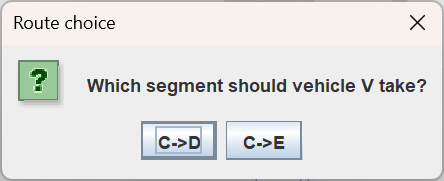
\includegraphics[scale=0.4]{../../screenshots/manual-controller-route.png}
		\caption{Route choice.}
		\label{fig:manual-controller-route}
	\end{figure}
	
	Figure~\ref{fig:manual-controller-demand} shows the input dialog for demand pickup decisions, which pops up when a vehicle arrives at the pickup location of an appeared and unserved demand.
	The dialog provides the name of the vehicle (\texttt{U} in the example), the data of the demand (i.e.\ the pickup location and earliest pickup time as well as the dropoff location and latest dropoff time), and the two choice buttons (i.e.\ yes and no).
	
	\begin{figure}[!ht]
		\centering
		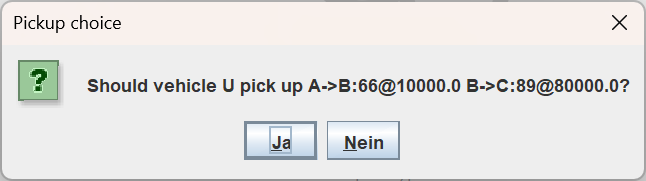
\includegraphics[scale=0.4]{../../screenshots/manual-controller-demand.png}
		\caption{Pickup choice.}
		\label{fig:manual-controller-demand}
	\end{figure}
	
	Figure~\ref{fig:manual-controller-charge} shows the input dialog for vehicle charging decisions, which pops up when a vehicle arrives at the location of an unoccupied charging station.
	The dialog provides the name of the vehicle (\texttt{U} in the example), the location of the charging station (\texttt{A->B:50} in the example), and the buttons for the two available choices (i.e.\ yes and no).
	
	\begin{figure}[!ht]
		\centering
		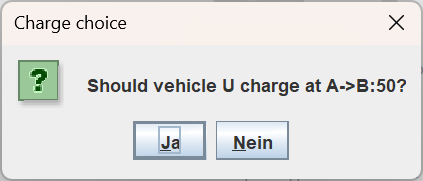
\includegraphics[scale=0.4]{../../screenshots/manual-controller-charge.png}
		\caption{Charge choice.}
		\label{fig:manual-controller-charge}
	\end{figure}
	
	Finally, the strategy always selects the maximum driving speed for each vehicle without considering possible collisions.
	And the strategy always chooses to fully charge the battery of each vehicle after the user decided to start the charging process.
	
	\subsubsection*{Random control strategy}
	\label{sec:controller-random}
	
	The random control strategy uses a standard random number generator for making the routing, demand pickup, and charging decisions described previously.
	For each decision, the strategy assigns equal probabilities to the available choices (i.e.\ outgoing segments of an intersection or yes and no).
	Furthermore, driving speed and target battery charge level are handled equally to the manual controller described in the previous section.
	
	\subsubsection*{Greedy control strategy}
	\label{sec:controller-greedy}
	
	The greedy control strategy uses a more sophisticated logic for determining routing decisions upon arrivals of vehicles at intersections of the driving infrastructure.
	The logic comprises four rules, which are processed in sequential order until one rule applies:
	\begin{enumerate}
		\item When the battery of the vehicle is only half full or less, the strategy randomly selects an outgoing road segment with charging station if such segment is avaiable.
		\item Then, when the vehicle carries one or more demands, the strategy randomly selects the drop-off segment of one such demand if reachable directly via the intersection.
		\item Next, when the vehicle carries no demand, the strategy randomly selects the pick-up segment of an unserved demand if reachable directly via the intersection.
		\item Finaly, when none of the above three rules apply, the strategy randomly selects any of the outgoing road segments of the current intersection with uniform probability distribution.
	\end{enumerate}
	Note that the above rules of the routing logic only consider the next segment and do not perform a look-ahead across more segments.
	Finally, the greedy control strategy always chooses to pick up demands or charge vehicle batteries if arriving at an unserved demand pick-up location or charging station.
	Also, the strategy always chooses to drive at maximum speed and to fully charge the batteries if a charging process has started.
	
	\subsubsection*{Smart control strategy}
	\label{sec:controller-smart}
	
	The smart control strategy uses an even more sophisticated strategy for determining routing decisions upon intersection arrivals of vehicles.
	The logic again comprises four rules, which are processed in sequential order until one rule applies:
	\begin{enumerate}
		\item When the vehicle carries one ore more demands and a charging station can be reached via their drop-off location, the segment leading to the closest such demand is selected.
		\item When the vehicle carries no demands and a charging station can be reached via the pick-up location of an unserved demand, the segment leading to the closest such demand is selected.
		\item When the vehicle carries no demands and does not plan to pick-up a new demand, the segment leading to the closest charging station is selected if reachable with the remaining battery level.
		\item Finally, when none of the above three rules apply, again the strategy randomly selects any of the outgoing road segments of the current intersection with uniform probability distribution.
	\end{enumerate}
	When arriving at an unused charing station, the smart control strategy only starts charging if no other charging station can be reached with the current battery level.
	Furthermore, when the charging station is used, but not other charging station can be reached, the strategy lets the vehicle wait at the station to become free.
	Finally, with this strategy vehicles always pick up unassigned demands when passing by, charge their batteries fully when at a charging station, and drive with maximum speed.
	
	\subsection{Data recorder}
	\label{sec:statistics-interface}
	
	During simulation, a number of events are recorded for visualization of system (and control strategy) performance as well as further processing such as strategy training.
	Figure~\ref{fig:statistics-interface} shows the provided methods of the data recorder interface.
	
	\begin{figure}[!ht]
		\centering
		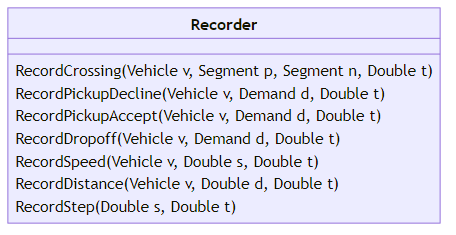
\includegraphics[scale=0.4]{../../diagrams/statistics/classes-v2.png}
		\caption{Statistics interface.}
		\label{fig:statistics-interface}
	\end{figure}
	
	The recorder tracks, when a vehicle crosses an intersection, and records the associated routing decision of the control strategy.
	Then, the recorder tracks, when a vehicle passes by an unassigned demand and the control strategy declines or accepts the pick up.
	Similarly, the recorder tracks, when a vehicle drops off a demand at its target location.
	Furthermore, the recorder continuously tracks the speed and the overall travel distance of the vehicles.
	Finally, the recorder also tracks the size of the time steps made during discrete event simulation.
	
	Currently, we use the data about intersection crossing for determining bottlenecks in the driving infrastructure.
	Also, we use the data about pick ups and drop offs for determining per demand waiting and driving as well as delays.
	In the future, we plan to add more recording capabilities as well as exploring additional use cases for the data.
	
	\subsection{Simulation engine}
	\label{sec:simulation-engine}

%	\begin{figure}[!ht]
%		\missingfigure{Simulation loop}
%		\caption{Simulation loop}
%	\end{figure}
	
	As explained previously, the simulation engine is responsible for computing event times, delegating control decisions to the control strategy, updating the model state, and dispatching relevant data to the recorder.
	The core of the simulation engine is the simulation loop, which advances the model time and updates the model state until no more events are to be processed.
	The simulation loop can be divided into three main steps:
	
	\paragraph{Step 1}
	
	%\textcolor{red}{TODO}
	Make routing decisions and update vehicle locations.
	Make charging decisions and update connections between vehicles and charging stations.
	Make pick up decisions, perform drop offs (also if vehicle battery empty), and update connections between vehicles and demands.
	Make speed decisions and update vehicle speeds.
	
	\paragraph{Step 2}
	
	%\textcolor{red}{TODO}
	Compute the time of the next event to be processed:
	Speed update timeout,
	charging speed update or charging station disconnect timeout,
	intersection arrival,
	charging station arrival,
	vehicle battery empty/full,
	demand appearance,
	demand overdue,
	demand pick up / drop off location arrival, and
	vehicle attach / detach.
	
	\paragraph{Step 3}
	
	%\textcolor{red}{TODO}
	Based on the current time and the time until the next event do the following:
	Update vehicle locations, vehicle battery levels, and record travelled distances of vehicles.
	Detect vehicle collisions based on their location, their width, and their overlaps along the segment line.
	Finally, set the model time to the time of the next event.
	
	\subsection{Specific applications}
	\label{sec:application}
	
	Based on the previous components we implemented two specific applications:
	The first application can be used for comparing the performance of different control strategies (see Section~\ref{sec:controller-comparison}).
	The second application can be used for comparing the performance of different driving and charging infrastructures as well as fleet configurations (see Section~\ref{sec:infrastructure-comparison}).

%	\subsubsection{Control strategy evaluation}
%	\label{sec:controller-evaluation}
%
%	\textcolor{red}{TODO}
	
	\subsubsection{Control strategy comparison}
	\label{sec:controller-comparison}
	
	To compare different control strategies, we apply these strategies to the same system configuration (including driving / charging infrastructure as well as fleet setup) and scenario (i.e.\ demand profile).
	For performance evaluation, we measure the times between demand appearances at the pick up location and subsequent disappearances at the drop off location.
	Figure~\ref{fig:controller-comparison} shows an example system configuration, on which the random, the greedy, and the smart control strategy are applied.
	
	\begin{figure}[!ht]
		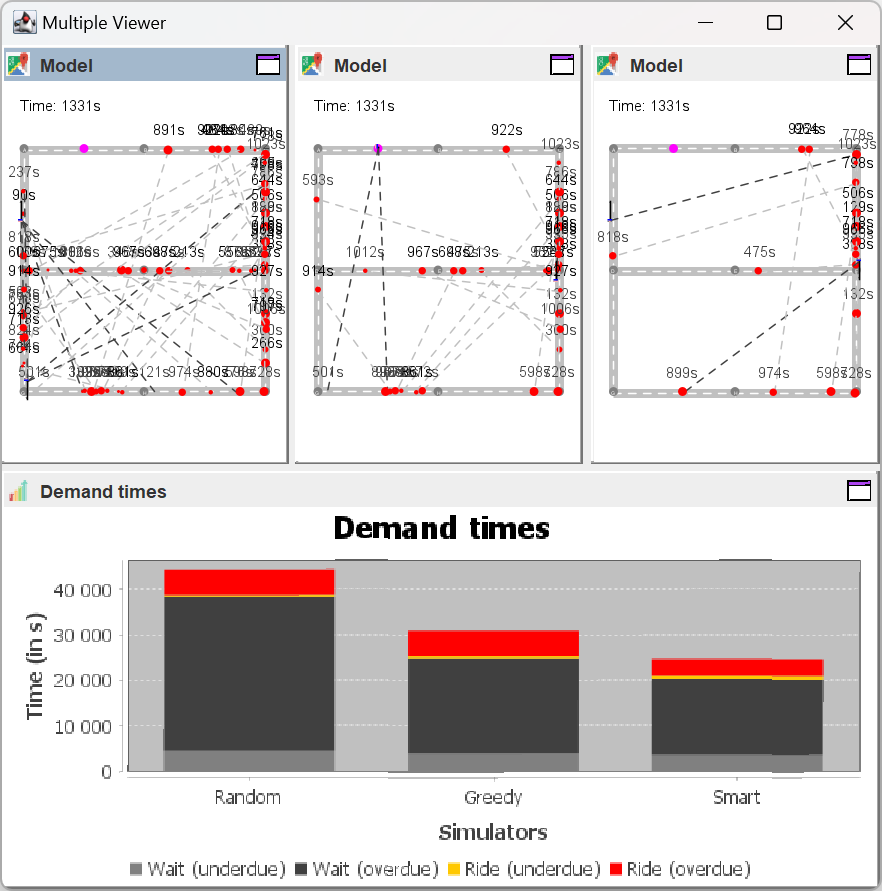
\includegraphics[width=\columnwidth]{controller_comparison.png}
		\caption{Control strategy comparison.}
		\label{fig:controller-comparison}
	\end{figure}
	
	The upper part of the window shows for each control strategy the current system state including the vehicle locations and the active demands.
	The lower part of the window shows for each control strategy the total times that have passed between demand appearances and their respective disappearances.
	From the diagram we can deduct that in this simulation run the smart control strategy showed superior performance over the others.
	Note that due to the random nature of the strategies, the result might have been very different in second run.
	
	\subsubsection{System configuration comparison}
	\label{sec:infrastructure-comparison}
	
	To compare system configurations, we instead apply the same control strategy and scenario (i.e.\ demand profile) to different versions of the driving / charging infrastructure as well as fleet setup.
	Note that different versions of the infrastructure might include additional road segments not present in others.
	Hence, we require that demands only reference road segments, which are included in every version of the driving infrastructure.
	Figure~\ref{fig:infratructure-comparison} shows an example of such system configuration comparison.
	
	\begin{figure}[!ht]
		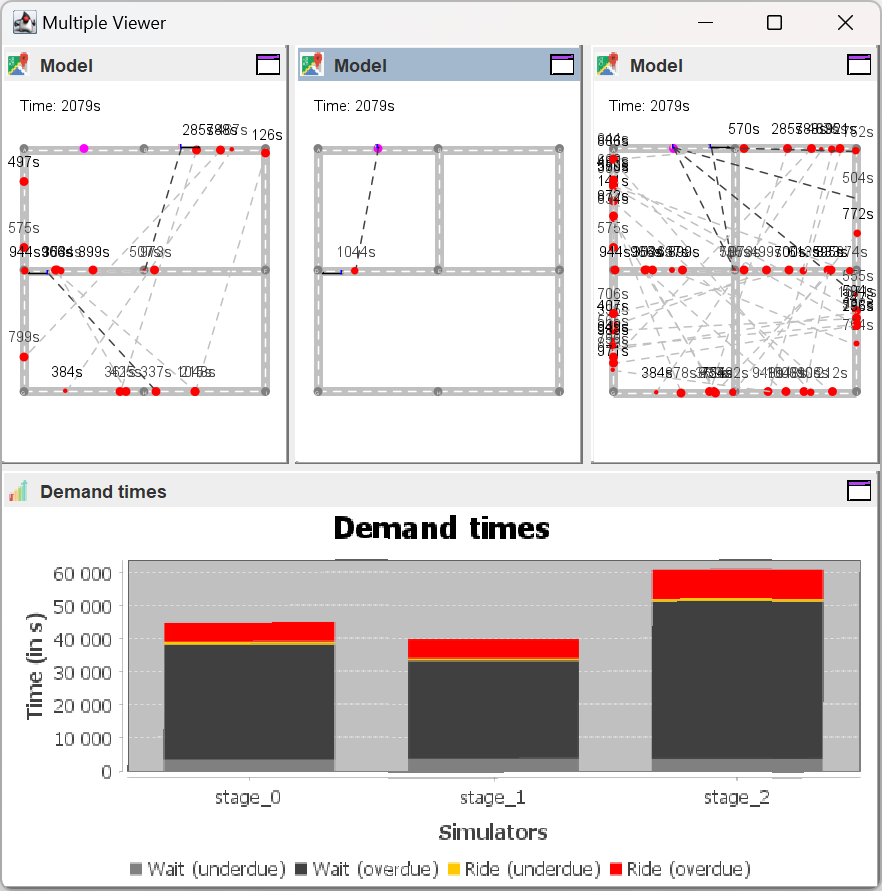
\includegraphics[width=\columnwidth]{infrastructure_comparison.png}
		\caption{System configuration comparison.}
		\label{fig:infratructure-comparison}
	\end{figure}
	
	Again, the upper part of the window shows for each control strategy the current system state including vehicle locations and demands.
	Also, the lower part of the window shows for each system configuration the total times between demand appearance and disappearance.
	In this simulation run, the system configuration in the middle, which adds only one additional road segment, has the best performance.
	This example mainly shows, that the smart control strategy not always delivers optimal results, which is necessary for a fair comparison of infrastructures.
	
	\section{Conclusion}
	\label{sec:conclusion}
	
	%Placeholder from abstract
Methods and tools are needed to explore the possible design space for emerging transportation paradigms, which support evaluation of system design alternatives and verification of system properties. In this work, we propose a modeling and simulation framework for capturing design decisions and evaluating emergent properties as well as control strategies for ITS design. In addition to capturing different design decisions, it assumes a user-centric perspective, where users can guide design decisions employing a novel user interface. We discuss and apply our modeling and simulation framework with respect to two specific applications.
	
	
	\bibliographystyle{apalike}
	{\small
		\bibliography{main}}
	
	
\end{document}

